% SPDX-License-Identifier: GPL-2.0-or-later
% Copyright 2018 Thibault Allançon

% !TEX encoding = UTF-8 Unicode
% $Header: /cvsroot/latex-beamer/latex-beamer/solutions/conference-talks/conference-ornate-20min.en.tex,v 1.6 2004/10/07 20:53:08 tantau Exp $

\documentclass[table]{beamer}

\usepackage{eso-pic}
\usepackage{color}
\usepackage{tikz}
\usepackage{wasysym}

\mode<presentation>
{
  \usetheme{Warsaw}
  %\usecolortheme[named=yellow]{structure}
  % or ...

  \setbeamercovered{invisible}
  % or whatever (possibly just delete it)
  
  \setbeamertemplate{navigation symbols}{}
  
  \newcommand*\oldmacro{}%
  \let\oldmacro\insertshorttitle%
  \renewcommand*\insertshorttitle{%
    \oldmacro\hfill%
    \insertframenumber\,/\,\inserttotalframenumber}
}


\usecolortheme{crane}

\usepackage{array}
\newcommand{\tabitem}{~~\llap{\textbullet}~~}
\newcolumntype{M}[1]{>{\centering\arraybackslash}m{#1}}
\newcolumntype{L}[1]{>{\centering\arraybackslash}l{#1}}
\usepackage{minted}

\usepackage[utf8]{inputenc}
% or whatever

\usepackage{times}
\usepackage{multirow}
\usepackage[T1]{fontenc}
\usepackage[french]{babel}
\usepackage{graphicx}


\renewcommand{\arraystretch}{1.5}

% Or whatever. Note that the encoding and the font should match. If T1
% does not look nice, try deleting the line with the fontenc.

\title[La baguette légendaire]{}

\titlegraphic{\raisebox{2em}{}}

\author[Prologin]{}

\date{}

\begin{document}

\begin{frame}
    %\vspace{+1cm}
    \centering 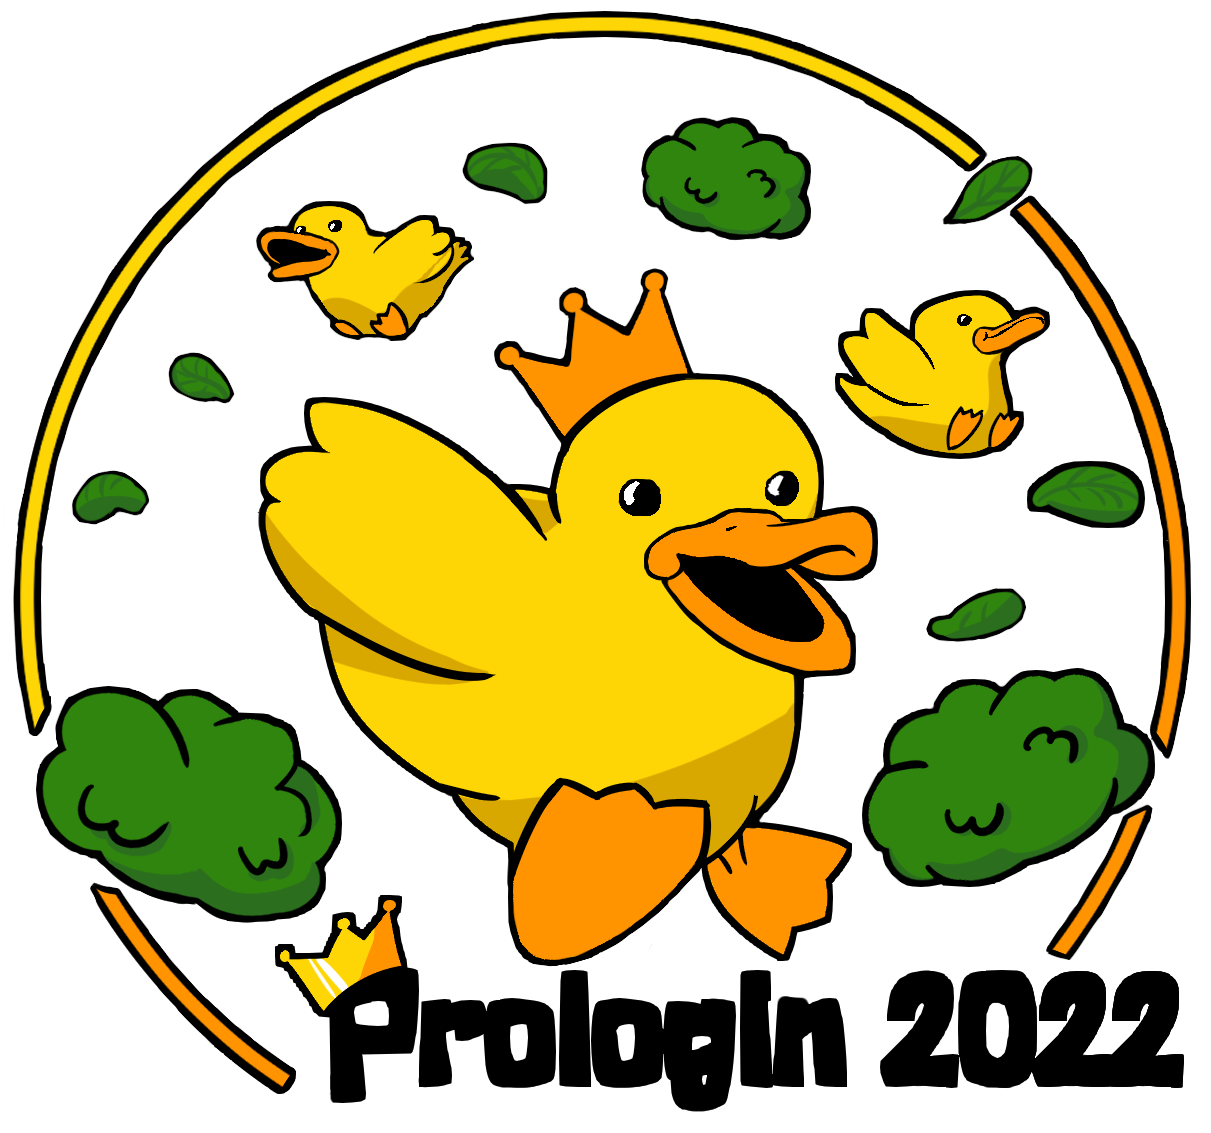
\includegraphics[width=0.7\linewidth]{img/logo-finale-2022.png}
\end{frame}

\begin{frame}
    %\frametitle{La marche des canards}
    % TOFIX PROLOGIN
    \Large
    \begin{center}
        La baguette légendaire\\
        \textbf{La marche des canards}
    \end{center}
    %\begin{block}{Objectifs}
    %    \begin{itemize}
    %        \item Être rentable
    %        \item Maximiser vos bénéfices 
    %        \item Obtenir \textbf{beaucoup} d'argent
    %    \end{itemize}
    %\end{block}
\end{frame}


\begin{frame}{L'objectif: le pain}
\centering

\includegraphics[width=5cm]{img/sprite/bread.png}
\end{frame}

\begin{frame}{La troupe canardienne}

    \begin{center}
    \begin{tabular}{p{1.5cm} c c c p{1.5cm}}
        Maman canard &&&& \footnotesize Vilain petit canard \\
        
\includegraphics[width=1.5cm]{img/sprite/ducks/duck_W_1.png} &
        
\includegraphics[width=1.5cm]{img/sprite/ducks/duckling_W_1.png} &
        
\includegraphics[width=1.5cm]{img/sprite/ducks/duckling_W_1.png} &
        
\includegraphics[width=1.5cm]{img/sprite/ducks/duckling_W_1.png} &
        
\includegraphics[width=1.5cm]{img/sprite/ducks/duckling_W_1.png} \\
        & antérieur &  $\Uparrow$   & postérieur &
        
    \end{tabular}
    \end{center}

\end{frame}


\begin{frame}
    \frametitle{La troupe}
     \begin{center}
        \begin{tabular}{c c}
            \begin{minipage}{0.4\textwidth}
            \centering
            
\includegraphics[width=0.6\textwidth]{img/sprite/ducks/duckling_S_1.png}
            \end{minipage}
             &
            \begin{minipage}{0.6\textwidth}
            \inputminted{cpp}{canard.cc}
            \end{minipage}
        \end{tabular}
     \end{center}
     
    %\small{Le butin ne peut pas être supérieur à \textbf{25} pièces d'or.}
\end{frame}

\begin{frame}{Les actions}
    \begin{center}
    \begin{tabular}{M{3cm} M{8cm}}
        Avancer &
        
\includegraphics[width=1cm]{img/sprite/ducks/duck_E_1.png} 
        
\includegraphics[width=1cm]{img/sprite/ducks/duck_W_1.png} 
        
\includegraphics[width=1cm]{img/sprite/ducks/duck_N_1.png} 
        
\includegraphics[width=1cm]{img/sprite/ducks/duck_S_1.png} \\
        Grandir & Ajouter un 
\includegraphics[width=1cm]{img/sprite/ducks/duckling_S_1.png} \\
        Construire un buisson & 
\includegraphics[width=1cm]{img/sprite/buisson.png} \\
        Creuser un tunnel & 
\includegraphics[width=1cm]{img/sprite/dirt.png} \\
    \end{tabular}
    \end{center}
\end{frame}

\begin{frame}
    \frametitle{Déplacement}
    Certaines cases sont traversables, d'autre non.
    \begin{center}
    \end{center}
    
    \begin{block}{Les points d'action restant en fin de tour !}
    Si une troupe n'a pas dépensé tous ses points d'action en fin de tour, la troupe avance dans sa direction actuelle, jusqu'à épuisement.
    \end{block}
\end{frame}

\begin{frame}
    \frametitle{Le parc}
    \begin{center}
        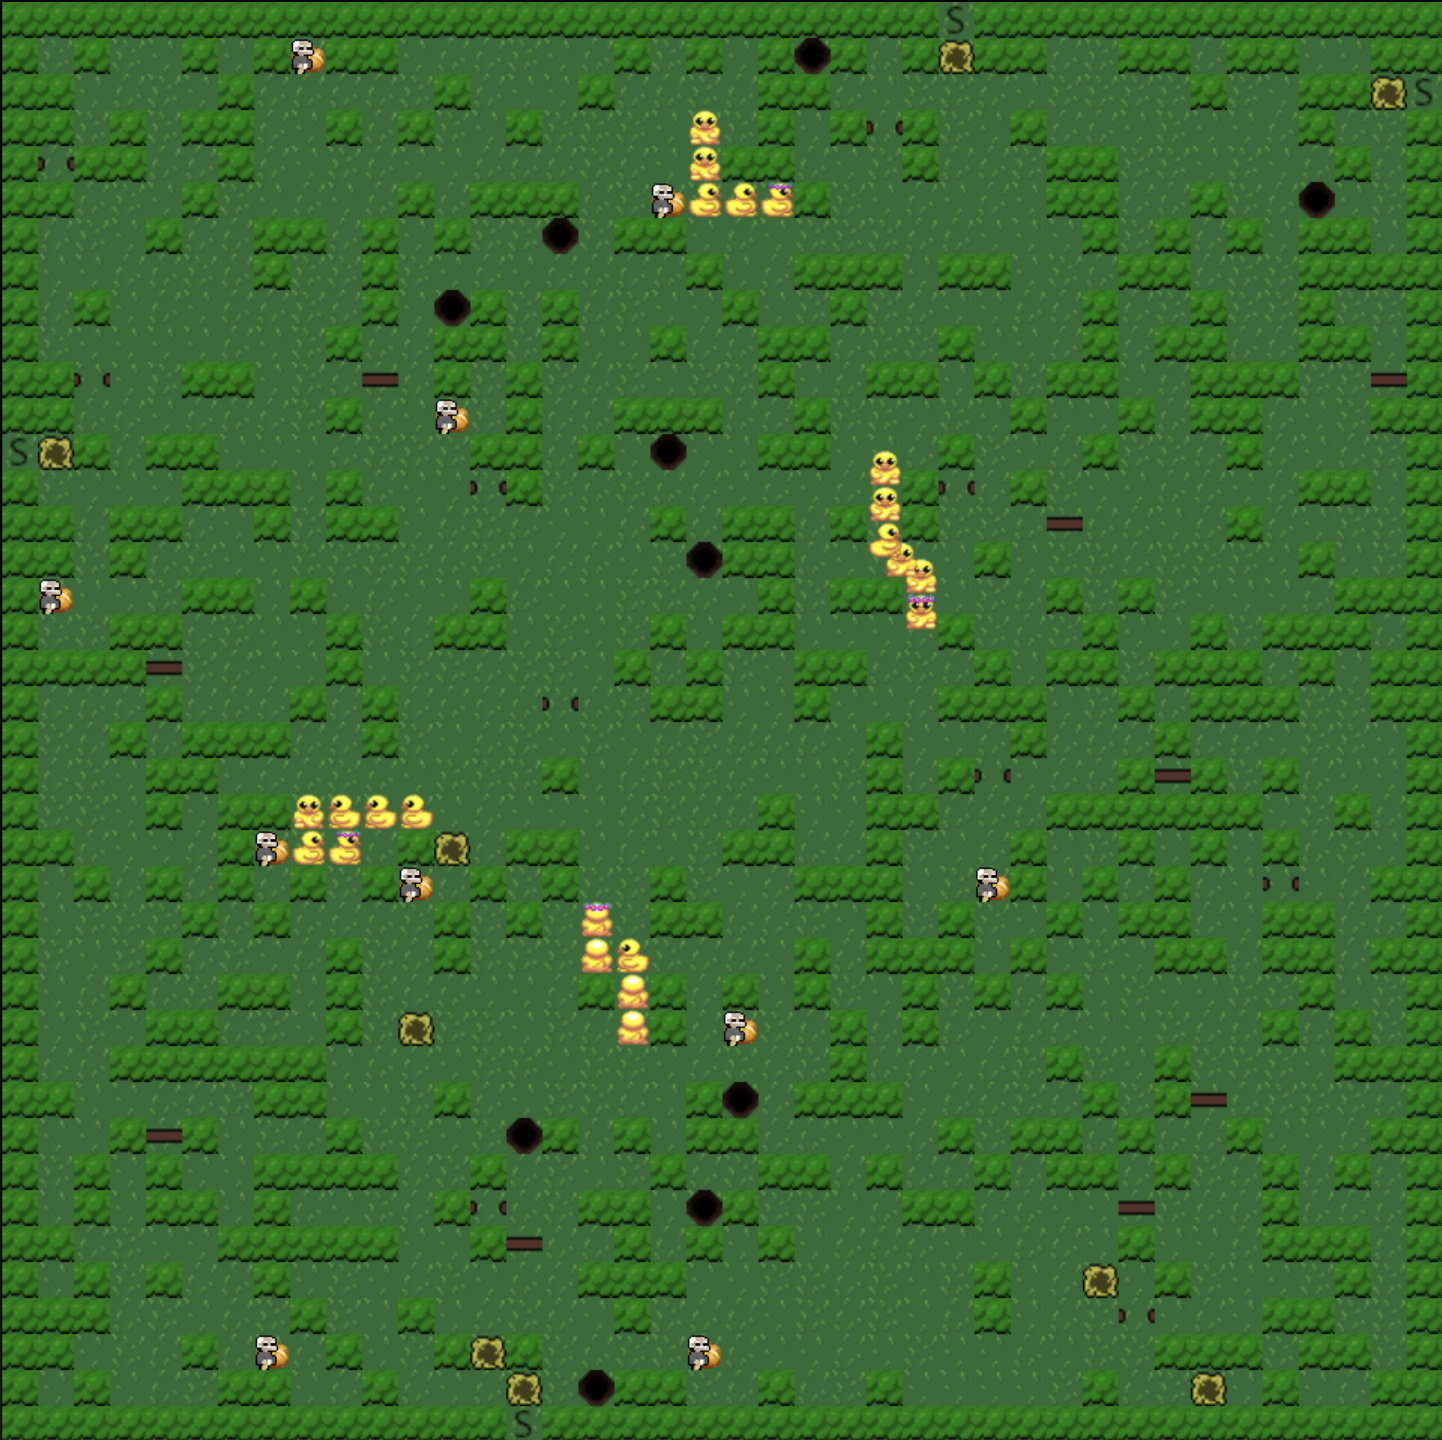
\includegraphics[width=0.7\textwidth]{img/map} 
    \end{center}
\end{frame}

\begin{frame}{Le parc}
    \begin{center}
    \begin{tabular}{l|c|l}
        \hline
        \textbf{Type} & \textbf{Échantillon} & \textbf{Représentation} \\
        \hline
        Gazon non constructible & 
\includegraphics[width=.5cm]{img/sprite/grass.png} & \texttt{' '} (un espace) \\
        Gazon & 
\includegraphics[width=.5cm]{img/sprite/grass.png} & \texttt{'.'} \\
        Point d’apparition & 
\includegraphics[width=.5cm]{img/sprite/spawn.png} & \texttt{'S'} \\
        Buisson & 
\includegraphics[width=.5cm]{img/sprite/buisson.png} & \texttt{'\#'} \\
        Barrière ouverte & 
\includegraphics[width=.5cm]{img/sprite/gate.png} & \texttt{'B'} \\
        Barrière fermée & 
\includegraphics[width=.5cm]{img/sprite/gate_close.png} & \texttt{'b'} \\
        Nid & 
\includegraphics[width=.5cm]{img/sprite/nest_empty.png} ou 
\includegraphics[width=.5cm]{img/sprite/nest_full.png} & \texttt{'N'} \\
        Papy & 
\includegraphics[width=.5cm]{img/sprite/papy.png} & entre \texttt{'0'} et \texttt{'9'} \\
        Trou & 
\includegraphics[width=.5cm]{img/sprite/trou.png} & \texttt{'X'} \\
        \hline
    \end{tabular}
    \end{center}
\end{frame}

\begin{frame}
    \frametitle{Le sous-terrain}
    \begin{center}
        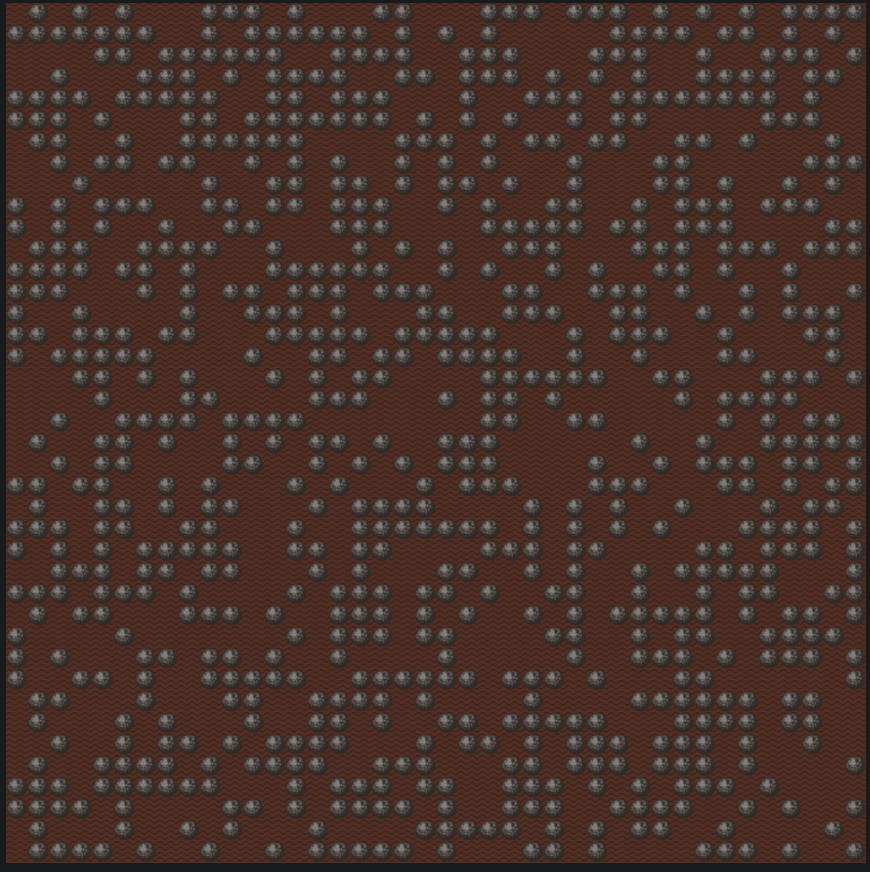
\includegraphics[width=0.7\textwidth]{img/under} 
    \end{center}
\end{frame}


\begin{frame}
    \frametitle{Pigeons de débug}
    \begin{columns}[T]
    \begin{column}{0.65\textwidth}
        \begin{itemize}
            \item Possibilité de placer des pigeons de débug sur n'importe quelle case
            \item Trois types : rouge, vert, bleu
            \item Aucune signification particulière, n'affecte pas la partie
            \item Complètement gratuit
        \end{itemize}
    \end{column}
    \begin{column}{0.45\textwidth}
        \centering
         \begin{minipage}{0.7\textwidth}
            
\includegraphics[width=\textwidth]{img/sprite/pigeon.png}
            \end{minipage}
    \end{column}
    \end{columns}    
\end{frame}

\begin{frame}
    %\frametitle{Exemple de simulation}
    \begin{center}
        \huge{Présentation des outils}
    \end{center}
\end{frame}


\begin{frame}
    \frametitle{Tournois intermédiaires}
    Trois fois par jours, prévus\footnote{Non contractuel} à :
    \begin{itemize}
        \item Vendredi 15 h 42 (tournoi de test)
        \item Vendredi 17 h 42
        \item Vendredi 23 h 42
        \item Samedi 5 h 42
        \item Samedi 11 h 42
        \item Samedi 17 h 42
    \end{itemize}
    Tournoi final (resultats à la remise des prix) \textbf{samedi à 23~h~42}.
\end{frame}


\begin{frame}
    %\frametitle{Questions}
    \begin{center}
        \huge{Des questions ?}
    \end{center}
    %Posez vos questions !
\end{frame}

\end{document}

%%%%%%%%%%%%%%%%%%%%%%%%%%%%%%%%%%%%%%%%%%%%%%%%%%%%%%%%%%%%%%%%%%%%%%%%%%%%%%%%%%%%%%%%%%%%%%%%%%%%%%%%%%%%%%%%%

\begin{frame}
    \frametitle{Les 6 nains}
     \begin{center}
        \begin{tabular}{c c}
            \begin{minipage}{0.5\textwidth}
            \includegraphics[width=\textwidth]{nain_bleu.png}
            \end{minipage}
             &
            \begin{minipage}{0.5\textwidth}
            \inputminted{cpp}{nain.cc}
            \end{minipage}
        \end{tabular}
     \end{center}
     
    \small{Le butin ne peut pas être supérieur à \textbf{25} pièces d'or.}
\end{frame}

\begin{frame}
    \frametitle{Aspects techniques}
    \begin{block}{Déroulement}
        \begin{itemize}
            \item \textbf{2} joueurs sont présents en même temps dans la mine.
    \item Simulation en tour par tour, un joueur contrôle ses 6 nains à chaque tour.
            \item Objectif : Rapporter plus de richesse à votre taverne que votre concurrent.
            \item Votre période d'évaluation est de \textbf{100 tours}
        \end{itemize}
    \end{block}
\end{frame}

\begin{frame}{Contrôles}
    \begin{tabular}{M{3cm} M{8cm}}
            \item Déplacer   
            &
            \includegraphics[width=2cm]{move_walk.png}
            \includegraphics[width=2cm]{move_climb.png}
            \includegraphics[width=1.5cm]{move_rope.png}
            \\
            \item Miner 
            &
            \includegraphics[width=5.5cm]{mine.png}
            \\
            \item Poser une corde
            &
            \includegraphics[width=1.8cm]{put_rope.png}
            \\
            \item Actionner une corde 
            &
            \includegraphics[width=1.6cm]{pull_rope.png}
    \end{tabular}
\end{frame}

\begin{frame}{Marcher}
    \begin{columns}[T]
    \begin{column}{0.5\textwidth}
         \includegraphics[width=\textwidth]{move_walk.png}
    \end{column}
    \begin{column}{0.5\textwidth}
        \large
         \begin{center}
            \begin{itemize}
                \item Coûte des PM
                \item 4 directions possibles
                \item Attention à la gravité !
            \end{itemize}
         \end{center}
    \end{column}
    \end{columns}
\end{frame}

\begin{frame}{Escalader}
    \begin{columns}[T]
    \begin{column}{0.5\textwidth}
         \includegraphics[width=\textwidth]{move_climb.png}
    \end{column}
    \begin{column}{0.5\textwidth}
        \large
         \begin{center}
            \begin{itemize}
                \item Coûte plus de PM
                \item 4 directions possibles
                \item Attention il faut s'accrocher !
            \end{itemize}
         \end{center}
    \end{column}
    \end{columns}
\end{frame}

\begin{frame}{Escalader sur une corde}
    \begin{columns}[T]
    \begin{column}{0.5\textwidth}
         \includegraphics[width=\textwidth]{move_rope.png}
    \end{column}
    \begin{column}{0.5\textwidth}
        \large
         \begin{center}
            \begin{itemize}
                \item Réduit le coût d'escalade
                \item 2 directions possibles pour rester sur la corde
                \item On peut se faire tracter
            \end{itemize}
         \end{center}
         \textbf{Poser une corde nécessitera tous les PA de toute l'équipe !}
    \end{column}
    \end{columns}
\end{frame}

\begin{frame}{Actionner une corde}
    \begin{columns}[T]
    \begin{column}{0.5\textwidth}
         \includegraphics[width=\textwidth]{pull_rope.png}
    \end{column}
    \begin{column}{0.5\textwidth}
        \large
         \begin{center}
            \begin{itemize}
                \item Coûte des PAs
                \item 2 directions possibles
                \item Bouge tous les nains sur la corde
            \end{itemize}
         \end{center}
    \end{column}
    \end{columns}
\end{frame}

\begin{frame}{Se marcher dessus}
\begin{center}
    \includegraphics[width=0.6\textwidth]{se_marcher.png}
\end{center}
\end{frame}

\begin{frame}
    \frametitle{Aspects techniques}
    \begin{block}{Points de déplacement}
        \begin{itemize}
            \item À chaque tour, tous les agents ont 5 points de déplacement
            \item Les points ne sont utilisables que pour le tour actuel
            \item Pas de transfert de points entre agents
        \end{itemize}
    \end{block}
    \begin{block}{Coût}
        \begin{itemize}
            \item Marcher : 1 point
            \item Escalader une paroi : 2 points
            \item Se déplacer le long d'une corde : 1 points
        \end{itemize}
    \end{block}
\end{frame}

\begin{frame}
    \frametitle{Aspects techniques}
    \begin{block}{Points de d'action}
        \begin{itemize}
            \item À chaque tour, les nains ont chacun 6 points d'action
            \item Les points ne sont utilisables que pour le tour actuel
            \item Pas de transfert de points entre nains
        \end{itemize}
    \end{block}
    \begin{block}{Coût}
    \begin{itemize}
            \item Miner : 6 points
            \item Tirer sur une corde : 1 point
            \item Poser une corde : tous les PAs de toute l'équipe (cas particulier)
        \end{itemize}
    \end{block}
\end{frame}

\begin{frame}
    \frametitle{Actions gratuites}
    \begin{tabular}{M{3cm} M{3cm} M{3cm}}
        \item  S'accrocher et tomber &
        \includegraphics[width=2cm]{move_climb.png} &  
        \includegraphics[width=2.2cm]{fall.png}
    \end{tabular}
   
    \begin{block}{Dégâts de chute}
        \begin{itemize}
            \item Le nain prend
            des dégâts relatifs à la hauteur de sa chute
            \item 0 pour une chute de $h \leq 3$ cases, $2^{h-4}$ pour une chute de $h \geq 4$ cases
            \item Un nain en chute libre tombe instantanément tout en bas
        \end{itemize}
    \end{block}
\end{frame}

\begin{frame}
    \frametitle{Gestion des points de vie}
    \begin{block}{Point de vie}
        \begin{itemize}
            \item Les nains sortent de la taverne avec 10 points de vie
            \item Il peuvent en perdre par une chute ou par coups de pioches
            \item Un coup de pioche sur une case avec plusieurs nains touche tous les nains
            \item Un coup de pioche fait perdre 3 points de vie
        \end{itemize}
        
    \end{block}
    \begin{center}
        \includegraphics[width=2.2cm]{hurt.png} 
    \end{center}
\end{frame}

\begin{frame}
    \frametitle{Gestion des points de vie}
    \begin{block}{Décès}
        \begin{itemize}
            \item Quand un nain arrive à 0 point de vie, il meurt
            \item Son butin disparaît en cas de mort par chute
            \item Son butin va au nain meurtrier en cas de coup de pioche
            \item Il ressort de sa taverne au tour suivant
            \item La taverne adverse est meurtrière
        \end{itemize}
    \end{block}
    \begin{center}
        \includegraphics[width=2.2cm]{dead.png} 
    \end{center}
\end{frame}

\begin{frame}
    \frametitle{Les Minerais}
    


    
    
    \begin{tabular}{c c}
        \begin{minipage}{0.5\textwidth}
          \small
          \begin{center}
            \begin{tabular}{r l c}
              & \textbf{Minerai} & \textbf{Rendement} \\
              \includegraphics[width=0.5cm]{frames/granit.png} & Granit & 0 \\
              \includegraphics[width=0.5cm]{frames/coal.png} & Charbon & 1 à 4 \\
              \includegraphics[width=0.5cm]{frames/iron.png} & Fer & 5 à 9 \\
              \includegraphics[width=0.5cm]{frames/or.png} & Or & 10 à 14 \\
              \includegraphics[width=0.5cm]{frames/diamonds.png} & Diamants & 15 à 19 \\
              \includegraphics[width=0.5cm]{frames/emerauld.png} & Émeraudes & 20 à $\infty$ \\
              \includegraphics[width=0.5cm]{frames/ruby.png} & Rubis & $\mathbb{Z}$ \\
            \end{tabular}
          \end{center}
        \end{minipage}
        \begin{minipage}{0.5\textwidth}
          \begin{itemize}
              \item Donner un coup de pioche coûte 6 points d'action
              \item Le nombre de coups de pioche nécessaires, et la valeur gagnée, dépendent de la position du bloc de pierre
          \end{itemize}
        \end{minipage}
    \end{tabular}
\end{frame}




\begin{frame}
    \frametitle{Fin}
    Nous vous souhaitons le meilleur rendement possible...
    \pause

    ... mais d'abord, \textbf{distribution de l'équipement} !
\end{frame}

